\chapter{Environment}
\label{chapter:environment}

% Most often you need to describe the environment you work in, what limits there are and so on. This is a good place to do that. Sometimes the environment is described together with your own implementation, in the same chapter.

% \emph{[ - Data and data preprocessing - , Audio, PIR, time/frequency domain, Mel-Frequency spectrum, MFCC, Data collection circumstances, Ground truth with camera]}
% \bigskip

In this chapter, we will give an overview of the basics of audio and PIR signal processing needed to understand the practical implementation of the multisensory prediction model. Since the goal is to classify different events, in the preprocessing step we aim to generate the most insightful but minimal set of features, from which presence can be easily detected. Our research will include time and frequency domain analysis of the audio signal and a basic introduction of the PIR sensor data.



\section{Raw PIR data processing}

Passive Infrared (PIR) sensors are the most widely used devices for motion detection and presence estimation for indoor spaces. Due to its simplicity, one sensor is incapable of distinguishing the source of movement or its direction. However, more options are available using analog sensors, since the sensitivity can be adjusted on the field for different applications and more information can be extracted from the signal waveform.

\subsection{The PIR sensor}
% TODO: better PIR sensor description Michrophonics: occupancy sensor technologies white paper pdf
 %PIR sensors are the most widely used devices for motion detection and presence estimation for indoor spaces. 
 The PIR sensor exploiting the pyroelectric properties of the applied materials, it can convert the absorbed infrared radiation into measurable analog voltage after a signal amplification step. 
 To be able to detect movement in the sensor field of view, PIR sensors split at least two parts and measure the relative difference between them canceling out the absolute radiation always present in the room. Additionally, focusing the IR rays to the different sensor elements, a custom-designed Fresnel lens is used, precisely controlling detection area and sensitivity. An example of a typical detection area arrangement for a ceiling-mounted PIR sensor can be seen in figure \ref{fig:pir_fov}. Sensor manufacturers are offering a wide variety of lenses tailor-made for the most common use cases ranging from horizontally wide detection areas for corridors to long-distance detection for sports halls with 7-10 meters expected installation height.

\begin{figure}[ht!]
  \begin{center}
    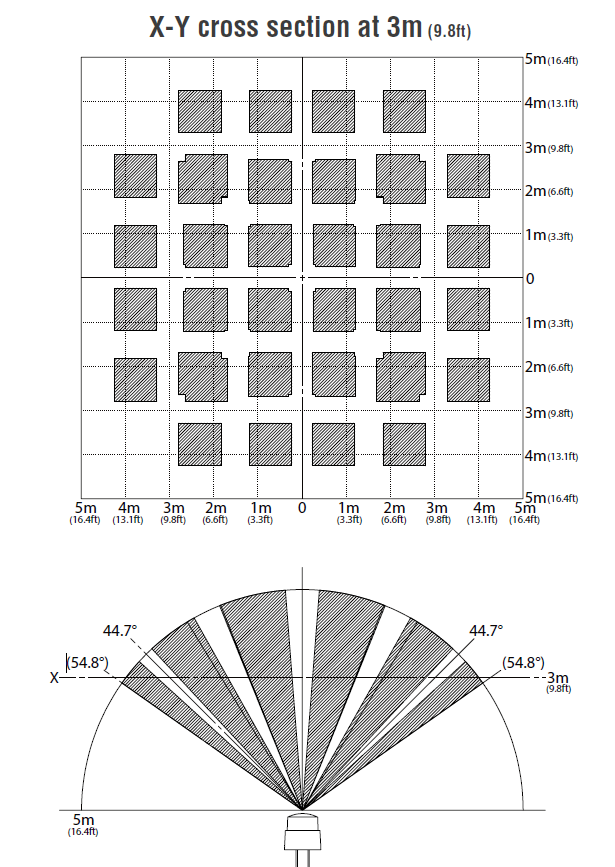
\includegraphics[width=0.5\textwidth]{thesistemplate/fig/pir_fov.png}
    \caption{Field of view of an industrial PIR sensor \cite{papir_dsheet}, the arrangement and sizes of detection zones are controlled by custom lens design.}
    \label{fig:pir_fov}
  \end{center}
\end{figure}

PIR sensors detect humans by their body temperature relative to the surrounding environment. As the thermal radiation for people mostly consists of infrared waves, it is sufficient to construct a sensor exclusively dedicated to spotting the IR level change in its switching zones. Sensor sensitivity can be increased by careful design of the lens, dividing the detection area into multiple smaller switching zones. Detection sensitivity is up to 4 \textdegree C at sensor level in most cases, between the background and the target object.


% JUHAA
%  You could also mention, that digital PIR variants often have integrated electronics providing output hold time (from seconds to minutes, configurable by user). This enables direct lighting control output.
From an application point of view, there are many variations of PIR sensors are available on the market. Starting from the most simple solution, analog PIR sensors provide direct access to the sensing elements with or without signal conditioning by an additional Amplifier circuit. To provide digital output, manufacturers integrate a Comparator circuit too after the signal amplification with a fixed threshold to distinguish between motion and steady-state. Moreover, the most complex digital PIR products offer adjustable sensitivity and output hold time with potentiometers. This way the signal output can be kept high for seconds or even minutes, which makes them applicable for direct lighting control without additional electronics.


Due to their physical properties, PIR sensors require a direct line of sight, which makes them hard to use in some special circumstances where people can be occluded by partitions or larger machines. Extensive deployment of single PIR sensors might mitigate the problem, but for a robust and flexible solution companies tend to deploy new approaches for more reliable presence detection.

%https://b2b-api.panasonic.eu/file_stream/pids/fileversion/4540
%https://na.industrial.panasonic.com/products/sensors/sensors-automotive-industrial-applications/lineup/pir-motion-sensor-papirs




\section{PIR based occupancy detection issues}

PIR or movement detection sensors are essential building blocks of automated lighting control systems. Unfortunately movement only is sometimes not sufficient to detect human presence, given the fact that PIR sensors are often not as sensitive to catch small changes in posture or breathing, therefore to avoid incorrectly turning the light off, they apply relatively long timeout values. 

Increasing the waiting time for new detected movement will improve system stability, but it also increases excess energy usage inevitably. By adjusting this interval the system can be tuned manually but due to the unpredictable nature of human activities, it falls far short of optimal behavior. Moreover, based on experience, PIR sensors can also produce false-positive triggers occasionally, due to various effects. Sudden changes in temperature, electromagnetic noises, or other building automation systems such as automatic window opening and curtain movements can trigger the sensor and lead to false lighting control scenarios. 


\begin{figure}[ht!]
  \begin{center}
    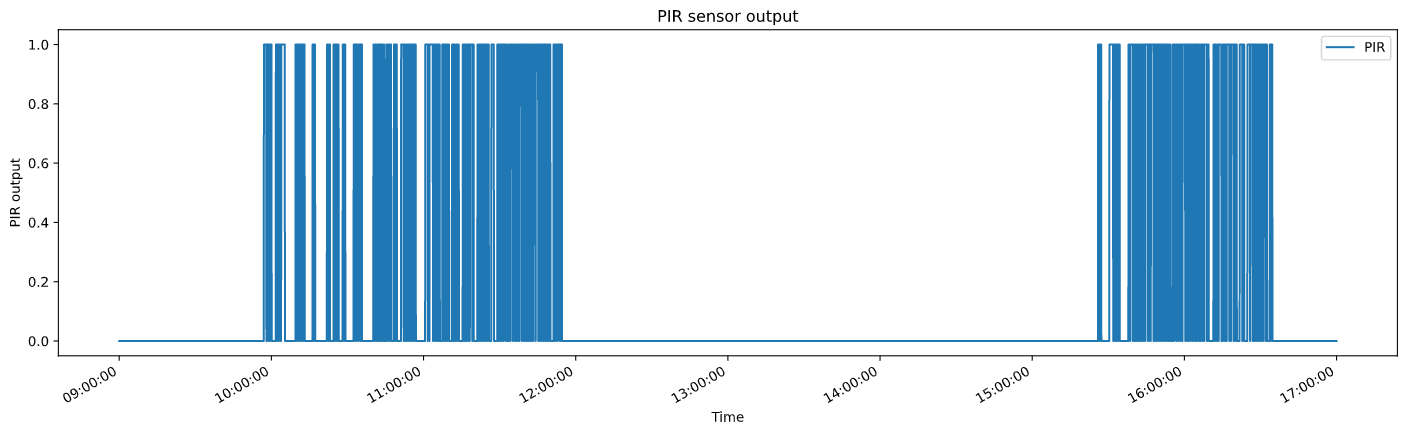
\includegraphics[width=1\textwidth]{thesistemplate/fig/pir_sensor_output.png}
    \caption{Raw output from a ceiling mounted PIR sensor during a working day, high output corresponds to detected movement.}
    \label{fig:state_mach}
  \end{center}
\end{figure}

% \subsection{PIR sensor output}

% Here we could display the difference between an analog and a digital PIR sensor output with a graph. The digital version mostly just a simplified version of the analog employing an amplifier and a comparator with a static threshold.

\section{Audio signal processing}

Audio signal processing is an engineering discipline concerned with the analog or digital manipulation of audio signals. To help to understand the implementation part of the thesis we only cover the most important concepts essential for comprehension.

\subsection{Audio signal}

After vision, the second most important sense humans rely on for information gathering from our closest environment is hearing. A sound signal is defined as sound pressure change over time, which propagates through a transmission medium. The generally accepted audio frequency range is 20 Hz to 20 kHz \cite{rosen2011signals_speech}, but studies show that the hearing sensitivity declines, especially in the upper-frequency range starting from early adulthood \cite{jilek2014hearing_loss}. 

Considering human sound-producing capabilities the organ larynx plays the most important role, and more strictly the vocal folds inside it \cite{rossing02the_science_of_sound}. The mass and length of vocal folds determine the typical or fundamental frequencies used in speech, which varies slightly between the sexes. Males use lower frequencies in general with a fundamental frequency around 110~Hz compare to 220~Hz with females and 300 Hz with children, but there is a high variance amongst individuals. \cite{rossing02the_science_of_sound} 

%JUHAA
% The Science of Sound. Rossing, Moore Wheeler, 3rd edition.
% Speech production, Chapter 15, Page 339:

% "The rate of vibration of the vocal folds is determined primarily by their mass and tension, although the pressure and velocity of the air do contribute in a smaller way. The vocal folds are typically longer and heavier in the adult male than in the female and, therefore, vibrate at a lower frequency (pitch). During normal speech, the vibration rate may vary over a 2:1 ratio (one octave), although the range of a singer's voice is more than two octaves. Typical frequencies used in speech are 110 Hz in the male, 220 Hz in the female and 300 Hz in the child, with wide variations from one individual to another."

The microphone is the most commonly used device to convert the sound pressure change into an electrical signal, firstly to a continuous analog signal then through sampling and discretization to digital audio. This step is inevitable in situations, where any kind of digital filtering or postprocessing is required for signal enhancement or manipulation.


\begin{figure}[ht!]
  \begin{center}
    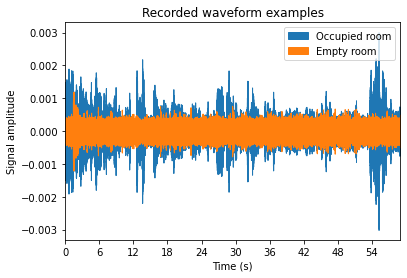
\includegraphics[width=0.6\textwidth]{thesistemplate/fig/recorded_waveform_ex.png}
    \caption{One minute normalized audio signal from empty and occupied room scenarios.}
    \label{fig:raw_aud_plot}
  \end{center}
\end{figure}


\subsection{Pulse Code Modulation}

Pulse code modulation (PCM) refers to a coding method used to transform analog waveforms to digital signals by sampling in time domain and quantization in value. Sampling frequency or sample rate determines the number of samples in one second, which reduces the continuous-time signal to a sequence of discrete values at specified time intervals. The selected sampling rate will affect the maximal bandwidth of the signal which can be reconstructed correctly without aliasing effects. According to the Nyquist Sampling Theorem, a continuous-time signal can be accurately reconstructed from its samples if the sampling frequency is at least twice as large as the highest frequency component.

\begin{equation*}
    f_{max} < f_s / 2
\end{equation*}

So choosing a sampling rate $f_s$ of 8 kHz will limit the signal to frequencies between 0 and 4 kHz. If the signal contains higher frequency components it needs to be filtered out by a low-pass filter to avoid aliasing effects.
%JUHAA
% Mention here Nyquist rate. Fs/2 gives upper limit of the signal frequency range. So 8kHz Fs means that signal can include frequencies in between 0 - 4kHz. If analog signal includes higher frequencies before AD, signals at higher frequencies will fold to lower frequencies. This is why signal should be always low-pass filtered before AD. MEMS mic with I2S output takes care of that for you.
The most commonly used sampling rates are 8000 Hz in telecommunication, 44,100 Hz as the standard CD quality, or 48000 Hz as audio channels for movies.


Although in some professional use cases might require an even higher sample rate in special circumstances. While in value, bit depth and the quantization levels  have to be defined. PCM as a general term is often used to describe LPCM or Linear pulse code modulation coding as the most commonly used  quantization method. LPCM features uniformly distributed levels for digitization purposes and the number of possible discrete values determined by the bit depth. The CD standard uses 16-bit resolution while modern digital media services apply 20, 24-bit depth for a bigger dynamic range representation.


\begin{figure}[ht!]
  \begin{center}
    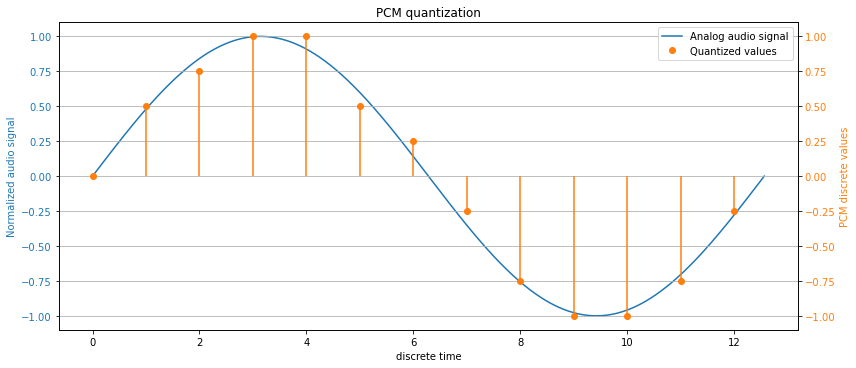
\includegraphics[width=0.9\textwidth]{thesistemplate/fig/pcm_plot.png}
    \caption{PCM quantization example, with linearly uniform quanization levels (LPCM).}
    \label{fig:pcm}
  \end{center}
\end{figure}



\subsection{Mel Frequency Cepstral Coefficients}

The Mel Frequency Cepstral Coefficients (MFCC) are short-term features dominantly used for speech recognition \cite{mfcc_logan2000mel}, speaker identification and proven to be beneficial for general audio processing purposes for Music Analysis or Genre Classification.

Figure \ref{fig:mfcc_proc} shows the process of the computation of the MFCC features for a given audio wave. The method aims to compress the speech-related information from the amplitude spectrum of the signal in a computationally efficient way, also taking into consideration the human perception of speech. The first step is to create fixed-size frames of the audio signal with the help of a windowing function, for speech detection purposes it usually means 20-30 ms wide segments with Hamming window. 
%JUHAA Why? If you mention it, describe it with a bit more details.
Hamming window has proven to reduce spectral leakage effects in the next DFT step \cite{mfcc_logan2000mel}. The leakage, appearance of high-frequency noises, occurs inevitably because of the edges created by framing the signal and the nonzero difference between the ends. The second problem can be thought of as a jump in value if we consider it from a Fourier-transformation point of view, which assumes a periodic extension of the signal.

\begin{figure}[t]
  \begin{center}
    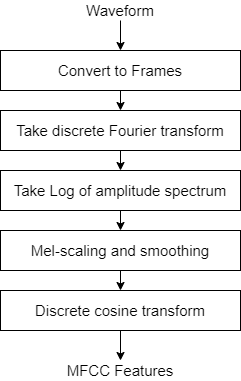
\includegraphics[width=0.25\textwidth]{thesistemplate/fig/mfcc_process.png}
    \caption{Process flow for generating MFCC features from audio signal, adapted from \cite{mfcc_logan2000mel}. }
    % https://ww2.mathworks.cn/help/audio/ref/mfcc.html
    \label{fig:mfcc_proc}
  \end{center}
\end{figure}

This step is followed by the Discrete Fourier Transformation of each frame to get the frequency spectrum representation of the signal from where the logarithm of the amplitude spectrum is extracted next. The logarithm function was applied because human loudness perception follows a quasi logarithmic scale. The phase information is not utilized for MFCC computation, previous research has shown few additional benefits compared to the computational overload.

After the scaled spectrum amplitude components the next step is to reduce the number of components by grouping and averaging them according to the Mel-scale. The Mel-scale is used to divide the whole frequency spectrum to the final number of MFCC bins by dedicating smaller intervals in the lower frequency range and increasing the size in a logarithmic manner mapping the human pitch perception. An example Mel-filter bank for computing 20 mels is depicted in \autoref{fig:mel_filter_bank}.

%JUHAA
% Can you give just a briefly more practical explanation why DCT is applied. The last step here calculates "the spectrum of the log of spectrum", so called cepstrum. It could be done with DFT again but DCT has benefits. See this:
%https://dsp.stackexchange.com/questions/31/how-do-i-interpret-the-dct-step-in-the-mfcc-extraction-process
Finally, a Discrete Cosine Transform (DCT) is applied to decorrelate the Mel-spectral components, increase noise tolerance and produce the final MFCC feature set. DCT is selected in contrast to DFT because the expected shape of the spectrum is a declining line approximately, which is hard to fit with a full cycle of sine waves with DFT, while DCT has cosines with a half-integer number of cycles too, and does not assume periodic extension of the signal. To compress the information but preserve the overall shape of the spectrum, the algorithm discards the higher coefficients and only selects the first (say) 20-40 values of the DCT function as a good representation of the signal.

% http://citeseerx.ist.psu.edu/viewdoc/download?doi=10.1.1.11.9216&rep=rep1&type=pdf
% https://wiki.aalto.fi/display/ITSP/Cepstrum+and+MFCC



\begin{figure}[ht]
  \begin{center}
    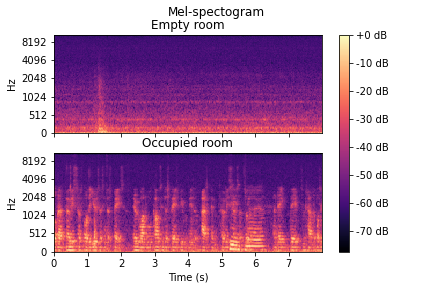
\includegraphics[width=0.8\textwidth]{thesistemplate/fig/mel_spec_comparison_ex.png}
    \caption{Mel-spectogram examples for short empty and occupied room recordings, the upper recording only had small noises from outside, while in the lower case represents an ongoing conversation.}
    \label{fig:mel_comp}
  \end{center}
\end{figure}


\begin{figure}[ht]
  \begin{center}
    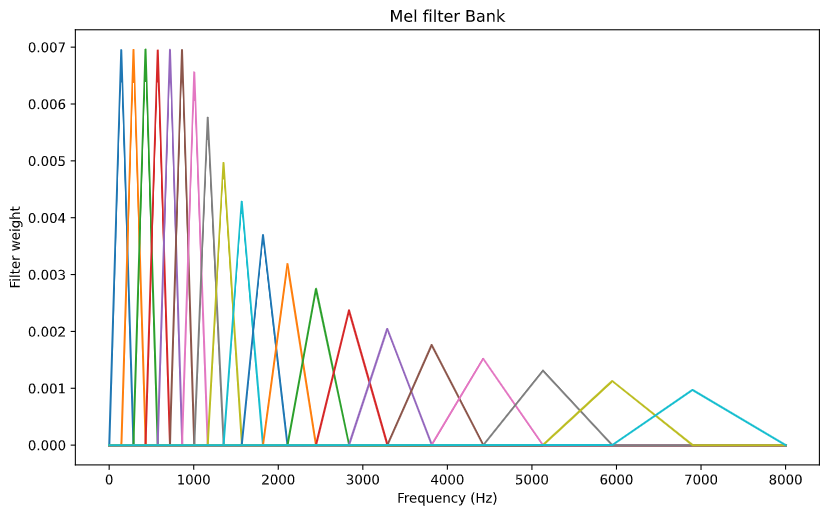
\includegraphics[width=0.8\textwidth]{thesistemplate/fig/mel_filter_bank.png}
    \caption{Mel-filter bank for 20 mels for 16 kHz sampling rate, each triangle represents the weighting values for the entire frequency spectrum, the peaks are constant until 1kHz and it decreases a logarithmic way for higher frequencies mimicking the human perception of sound.}
    \label{fig:mel_filter_bank}
  \end{center}
\end{figure}



 
%  Digital Signal Processing introduction contents:
%  \begin{itemize}
%   \item PCM, sample-rate - ok
%   \item Fourier transformation
%   \item Mel frequency spectrum/ MFCC - ok
%   \item Short time energy (STE), dBFS - decibels relative to full scale
%   \item Windowing, feature engineering
% \end{itemize}




% PDF\@.
% Comment: If your sentence ends in a capital letter, like here, you should
% write \@ before the period; otherwise LaTeX will assume that this is not
% really an end of the sentence and will not put a large enough space after the
% period. That is, LaTeX assumes that you are (for example), enumerating using
% capital roman numerals, like I. do something, II. do something else. In this
% case, the periods do not end the sentence.

% Similarly, if you do need a normal space after a period (instead of
% the longer sentence separator), use \  (backslash and space) after the
% period. Like so: a.\ first item, b.\ second item.

